\section{Background}
\label{sec:background}

Researchers have developed and improved several techniques to model users for 
the past 20 years~\citep{petrelli_user_centered_1999}~\citep{fink_adaptable_1997}. 
Modelling users needs to gather knowledge about their capabilities, drawbacks 
and limitations. During these first decades there was not any official and 
medical-based study to consult about user capabilities. Nevertheless, in 2001 
this situation changed. Under the \ac{who} coordination the World Health Assembly 
published the \ac{icf}\footnote{http://www.who.int/classifications/icf/en/} 
document. \ac{icf} is a classification of human functioning and disability. It 
classifies every function state associated with health (e.g., diseases, 
disruptions, injuries and traumas). Its purpose is to identify the low-level 
capabilities relevant to product design in several domains. As was written by 
experts in the area, the \ac{icf} document is a reference for identifying several 
user capabilities in any interaction process. Its goals are the following:

\begin{itemize}
  \item To provide a scientific basis for understanding and studying health and
  health-related states, outcomes and determinants.
  \item To establish a common language for describing health and health-related 
  states in order to improve communication between different users, such as health 
  care workers, researchers, policy-makers and the public, including people with 
  disabilities.
  \item To permit comparison of data across countries, health care disciplines,
  services and time.
  \item To provide a systematic coding scheme for health information systems.
\end{itemize}

\ac{icf} is organized into two main groups. Part 1 deals with \textit{Functioning 
and Disability}, including:

\begin{itemize}
  \item \textit{Body functions}, which are the physiological functions of body systems 
  (including psychological functions). It encompasses:
    \begin{itemize}
      \item Mental functions.
      \item \textit{Sensory functions and pain}.
      \item Voice and speech functions.
      \item \textit{Neuromusculoskeletal and movement-related functions}.
    \end{itemize}
  \item Body structures, as the anatomical parts of the body such as organs, 
  limbs and their components.
  \item Activities and participation. An activity is defined as the execution of 
  a task or action by an individual. Participation is involvement in a life 
  situation.
  \item Environmental factors, which make up the physical, social and attitudinal
  environment in which people live and conduct their lives.
\end{itemize}

It is important to remark the definition the \ac{icf} gives for \textit{impairment}:

\begin{description}
  \item[\Defi{Impairments}] \hfill \\
    \begin{mdframed}[hidealllines=true,backgroundcolor=gray!20]
    \textit{``Impairments are problems in body function or structure such as a 
    significant deviation or loss''.}
    \end{mdframed} 
\end{description}

On the other hand, Part 2 covers \textit{Contextual Factors}. This group gathers 
a list of \textit{Environmental Factors} which have an impact on all components 
of functioning and disability. A definition is given by \ac{icf}:

\begin{description}
  \item[\Defi{Environmental factors}] \hfill \\
    \begin{mdframed}[hidealllines=true,backgroundcolor=gray!20]
    \textit{``Environmental factors make up the physical, social and attitudinal
    environment in which people live and conduct their lives''.}
    \end{mdframed} 
\end{description}

\textit{Environmental factors} includes:

\begin{itemize}
  \item Products and technology.
  \item \textit{Natural environment and human-made changes to environment.} It 
  encompasses:
  \begin{itemize}
    \item Physical geography.
    \item Population.
    \item Flora and fauna.
    \item \textit{Climate}.
    \item Natural events.
    \item Human-caused events.
    \item \textit{Light}.
    \item \textit{Time-related changes}.
    \item \textit{Sound}.
    \item \textit{Vibration}.
    \item Air quality.
  \end{itemize}

  \item Support and relationships.
  \item Attitudes.
  \item Services, systems and policies.
\end{itemize}


This dissertation considers components under both parts. The description of each
component is detailed in Table~\ref{tbl:icf}.

\begin{table}
  \caption{\ac{icf} components considered in this dissertation.}
  \label{tbl:icf}
  \footnotesize
  \centering
  \begin{tabular}{l l l l}
    \hline
    \textbf{Category} 	& \textbf{Component group}& \textbf{Function}& \textbf{Description}\\
    \hline
    Body functions& Seeing and 	 	& Visual 	& Seeing functions of sensing	\\
    (Part I)	& related		& acuity	& form and contour, both 	\\
		& functions		& 		& binocular and monocular, for 	\\
		& 			& 		& both distant and near vision.	\\
		& Hearing and 		& Hearing 	& Sensory functions relating to \\
		& vestibular		& 		& sensing the presence of sounds\\
		& functions		& 		& and discriminating the location,\\
		& 			&		& pitch, loudness and quality of\\
		&			&		& sounds.			\\
		& Neuromusculos- 	& Mobility	& Functions of the range and ease\\ 
		& keletal and 		& of joint	& of movement of a joint.	\\
		& movement-related 	& 		& 				\\
		& functions		&		&				\\
    \hline
    Natural 	& Climate		& Temperature	& Meteorological features and 	\\
    environment & 			& Precipitation	& events, such as the weather.	\\
    and human-	&			& Wind		& 				\\
    made changes& Natural events	& 		& Geographic and atmospheric 	\\
    to environment& 			& 		& changes that cause disruption \\
    (Part II)	& 			& 		& in an individual's physical 	\\
		& 			& 		& environment			\\
		& Light			& Intensity	& Level or amount of energy 	\\
		& 			& 		& being emitted by either a 	\\
		& 			& 		& natural or an artificial source\\
		& 			& 		& of light.			\\
		& Time-related 		& 		& Natural, regular or predictable\\
		& changes		& 		& temporal change.		\\
		& Sound			& Intensity	& Level or volume of auditory 	\\
		& 			& 		& phenomenon determined by the	\\
		& 			& 		& amount of energy being generated.\\
    \hline
  \end{tabular}
\end{table}

First, the \textit{sensory 
functions} under the \textit{body functions} category of Part 1 are as the reference for adapting the user interface.


% \ac{icf} provides a multi-perspective approach to the classification of functioning 
% and disability as an \textit{interactive} and \textit{evolutionary} process. It 
% provides the building blocks for users who wish to create models and study 
% different aspects of this process. The interaction of the components remarked by
% \ac{icf} are illustrated in Figure~\ref{fig:icf_interaction}.
% 
% \begin{figure}
% \centering
% 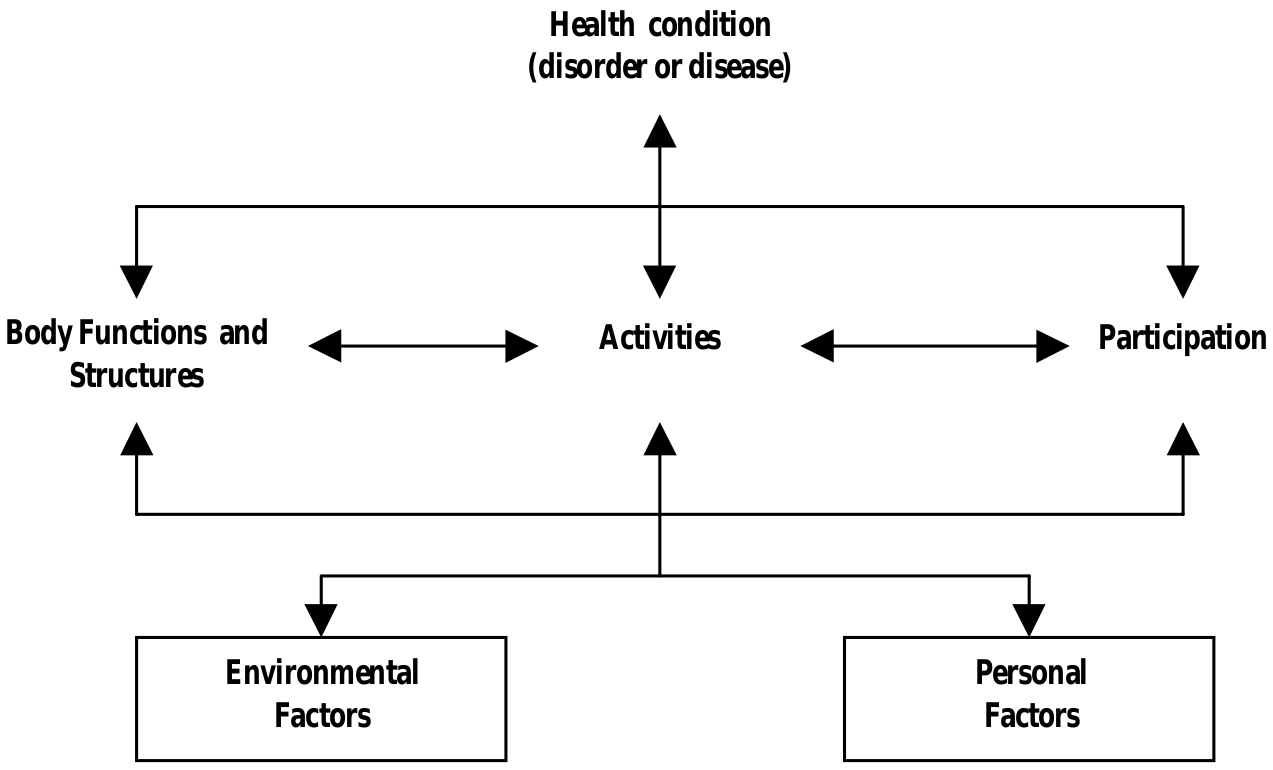
\includegraphics[width=0.75\textwidth]{icf_interaction.png}
% \caption{Interactions between the components of~\ac{icf}.}
% \label{fig:icf_interaction}
% \end{figure}